\section{Results}
\label{sec:results}

We present the three experiments in turn. Read together, the internal probe (\secref{sec:res2})
explains the behavior seen in reactivity (\secref{sec:res1}) and uncertainty
(\secref{sec:res3}): \emph{the base model encodes its answer in the prompt, and everything
else follows.}

\subsection{Experiment 1: reactivity to new information}
\label{sec:res1}

\Tabref{tab:exp1_change} reports the turn-1$\rightarrow$turn-2 answer change rate on \arc.
The base model barely revises, and it \emph{almost entirely ignores a genuinely informative
hint} appended after its answer: a $2\%$ change rate under \hint, versus $47\%$ for both
post-trained models. Fisher exact tests confirm the gap is enormous: \base versus \instruct
and \base versus \rlm differ at $p=2.6\times10^{-13}$ and $3.1\times10^{-10}$ under \generic,
and at $p=4.3\times10^{-28}$ and $3.8\times10^{-27}$ under \hint. Post-training does not make
models more rigid; it makes them \emph{far more} willing to revise.

\begin{table}[t]
    \centering
    \caption{Experiment~1, \arc ($N=200$). Turn-1$\rightarrow$turn-2 answer \textbf{change
    rate} by feedback type, with bootstrap 95\% CIs, and turn-1 accuracy. The base model is
    the most rigid on every feedback type and essentially ignores a genuine \hint. Most
    rigid (lowest change) per column in \textbf{bold}.}
    \label{tab:exp1_change}
    \begin{tabular}{@{}lccccc@{}}
        \toprule
        \textbf{Model} & \textbf{Turn-1 acc} & \textbf{\generic} & \textbf{\challenge} & \textbf{\hint} \\
        \midrule
        \base     & 0.65 & \textbf{0.17} {\scriptsize [.12,.22]} & \textbf{0.43} {\scriptsize [.35,.50]} & \textbf{0.02} {\scriptsize [.01,.04]} \\
        \instruct & 0.72 & 0.52 {\scriptsize [.44,.59]} & 0.56 {\scriptsize [.49,.64]} & 0.47 {\scriptsize [.40,.54]} \\
        \rlm      & 0.37 & 0.47 {\scriptsize [.41,.53]} & 0.43 {\scriptsize [.36,.50]} & 0.46 {\scriptsize [.39,.54]} \\
        \bottomrule
    \end{tabular}
\end{table}

\para{How each model reacts.} The change rate hides the \emph{direction} of revision, which
\tabref{tab:exp1_flip} and \figref{fig:exp1} make explicit. \instruct (plain RLHF)
\emph{over-reacts}: under content-free pushback it flips correct$\rightarrow$incorrect 33\% of
the time (38\% under \challenge)---textbook sycophancy. The reasoning model is the most
\emph{selective} reactor: it fixes wrong answers far more than it breaks correct ones,
especially given a hint ($\Delta^{i\rightarrow c}=0.30$ versus $\Delta^{c\rightarrow i}=0.08$).
The base model does neither, because it barely moves at all.

\begin{table}[t]
    \centering
    \caption{Experiment~1, \arc directional flip rates. $\Delta^{i\rightarrow c}$ is
    beneficial (wrong corrected to right); $\Delta^{c\rightarrow i}$ is harmful over-reaction
    (right broken to wrong). \instruct over-reacts under content-free \generic
    ($\Delta^{c\rightarrow i}=0.33$, \textbf{bold}); \rlm is selective, fixing more than it
    breaks under \hint.}
    \label{tab:exp1_flip}
    \begin{tabular}{@{}lcccc@{}}
        \toprule
        & \multicolumn{2}{c}{\textbf{\generic}} & \multicolumn{2}{c}{\textbf{\hint}} \\
        \cmidrule(lr){2-3} \cmidrule(lr){4-5}
        \textbf{Model} & $\Delta^{i\rightarrow c}$ & $\Delta^{c\rightarrow i}$ & $\Delta^{i\rightarrow c}$ & $\Delta^{c\rightarrow i}$ \\
        \midrule
        \base     & 0.06 & 0.04 & 0.02 & 0.00 \\
        \instruct & 0.11 & \textbf{0.33} & 0.25 & 0.20 \\
        \rlm      & 0.24 & 0.11 & \textbf{0.30} & 0.08 \\
        \bottomrule
    \end{tabular}
\end{table}

\begin{figure}[t]
    \centering
    \begin{subfigure}[b]{0.48\textwidth}
        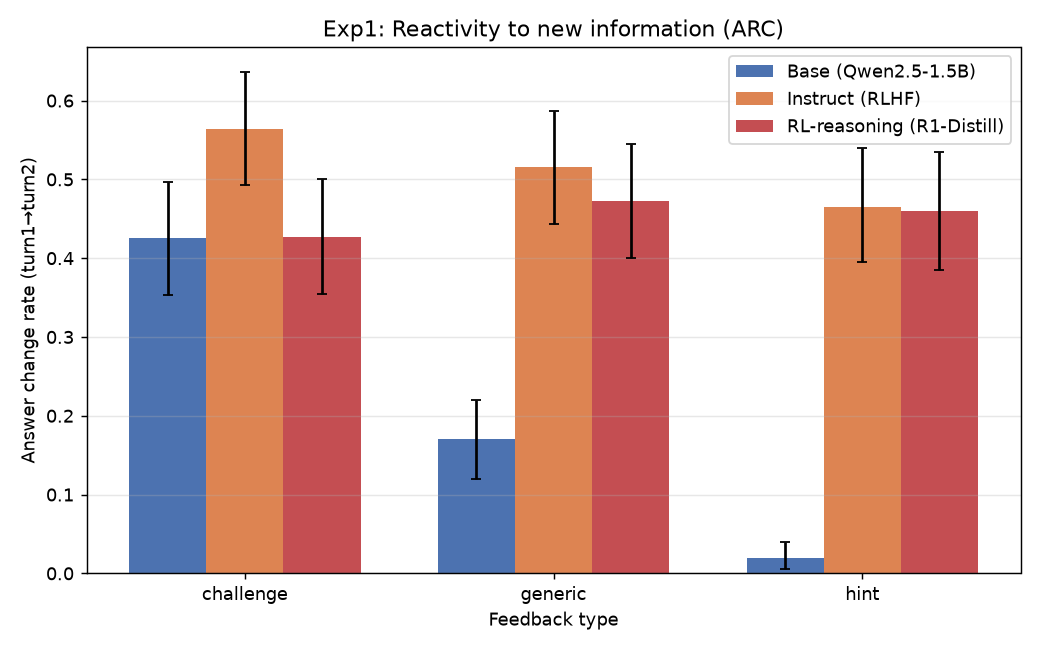
\includegraphics[width=\textwidth]{figures/exp1_reactivity_arc.png}
        \caption{Answer change rate by feedback type.}
        \label{fig:exp1_react}
    \end{subfigure}
    \hfill
    \begin{subfigure}[b]{0.48\textwidth}
        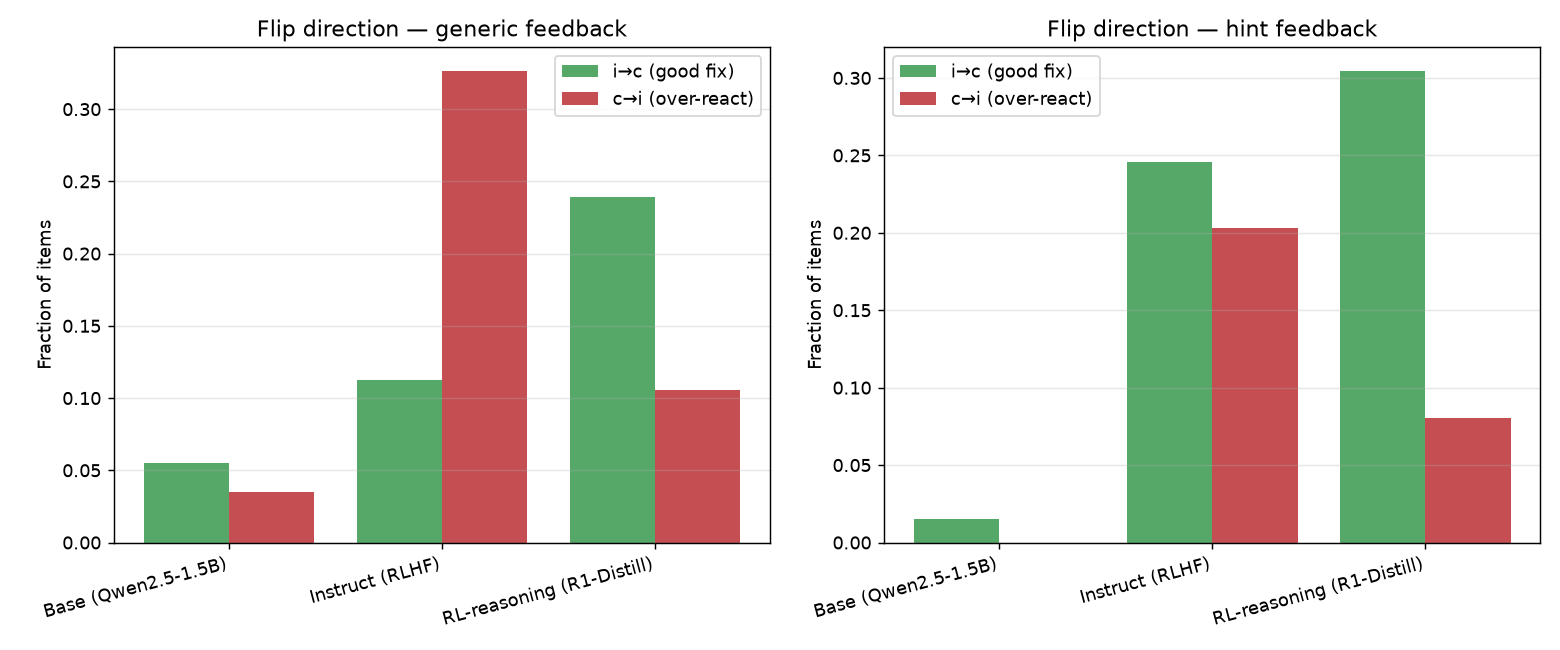
\includegraphics[width=\textwidth]{figures/exp1_flipdir_arc.png}
        \caption{Directional flip rates ($i\!\rightarrow\!c$ vs $c\!\rightarrow\!i$).}
        \label{fig:exp1_flip}
    \end{subfigure}
    \caption{Experiment~1 on \arc. \figleft The base model barely revises and ignores a
    genuine \hint, while both post-trained models revise about half the time. \figright The
    \emph{direction} differs: \instruct breaks correct answers under content-free pushback
    (over-reaction), whereas \rlm preferentially fixes wrong answers (selective reaction).}
    \label{fig:exp1}
\end{figure}

\para{Robustness on \gsm.} \Tabref{tab:exp1_gsm} repeats the experiment on numeric math.
Turn-1 accuracy now favors the math-distilled reasoning model (\rlm $0.77$, \instruct $0.67$,
\base $0.22$). Two findings emerge. First, the \emph{base model is rigid on both tasks}---the
single most consistent result across the paper. Second, the \emph{direction} of
post-training's reactivity effect is task- and correctness-dependent: here the high-accuracy
reasoning model \emph{over-reacts}, re-deriving and breaking its mostly-correct solutions
under content-free pushback ($\Delta^{c\rightarrow i}$ of $0.35$--$0.39$), the mirror image of
its selective behavior on \arc. Fisher tests put \base/\instruct versus \rlm at
$p\leq5.5\times10^{-12}$ on every condition, while \base versus \instruct is not significant
($p>0.3$). Because the \gsm hint is non-informative, this task isolates reaction to
content-free feedback.

\begin{table}[t]
    \centering
    \caption{Experiment~1 robustness on \gsm ($N=150$). All three feedback types are
    effectively content-free here. The base and instruct models are both rigid; the
    math-distilled \rlm over-reacts, breaking correct solutions ($\Delta^{c\rightarrow i}$
    $0.35$--$0.39$). Lowest change per column in \textbf{bold}.}
    \label{tab:exp1_gsm}
    \begin{tabular}{@{}lccccc@{}}
        \toprule
        \textbf{Model} & \textbf{Turn-1 acc} & \textbf{\generic} & \textbf{\challenge} & \textbf{\hint$^\ast$} & \textbf{Dominant flip} \\
        \midrule
        \base     & 0.22 & \textbf{0.15} & \textbf{0.13} & \textbf{0.08} & --- (rigid) \\
        \instruct & 0.67 & 0.16 & 0.18 & 0.07 & --- (rigid) \\
        \rlm      & 0.77 & 0.57 & 0.51 & 0.56 & $c\!\rightarrow\!i$ 0.35--0.39 \\
        \bottomrule
    \end{tabular}
\end{table}

\subsection{Experiment 2: the answer is pre-encoded---in the base model}
\label{sec:res2}

\Tabref{tab:exp2} reports the central mechanistic result. A probe predicting each model's
\emph{own} final answer from its prompt hidden state reaches $0.873$ balanced accuracy for the
base model---more than three times chance---falling to $0.712$ for instruct and to near-chance
$0.331$ for the reasoning model. The ordering is monotonic and inverts the hypothesis:
\emph{more post-training means the answer is committed later, not earlier.}

\begin{table}[t]
    \centering
    \caption{Experiment~2, \arc ($N=440$; four-way chance $=0.25$). Probe balanced accuracy
    predicting the model's \emph{own} final answer from the prompt-end hidden state (best
    layer), and self-consistency (own answer vs gold). The base model pre-encodes its answer
    (\textbf{0.873}); the reasoning model does not (\textbf{0.331}, near chance). Most
    pre-encoded in \textbf{bold}.}
    \label{tab:exp2}
    \begin{tabular}{@{}lcc@{}}
        \toprule
        \textbf{Model} & \textbf{Prompt-position acc} & \textbf{Self-consistency (vs gold)} \\
        \midrule
        \base     & \textbf{0.873} & 0.67 \\
        \instruct & 0.712 & 0.68 \\
        \rlm      & 0.331 & 0.39 \\
        \bottomrule
    \end{tabular}
\end{table}

\begin{figure}[t]
    \centering
    \begin{subfigure}[b]{0.48\textwidth}
        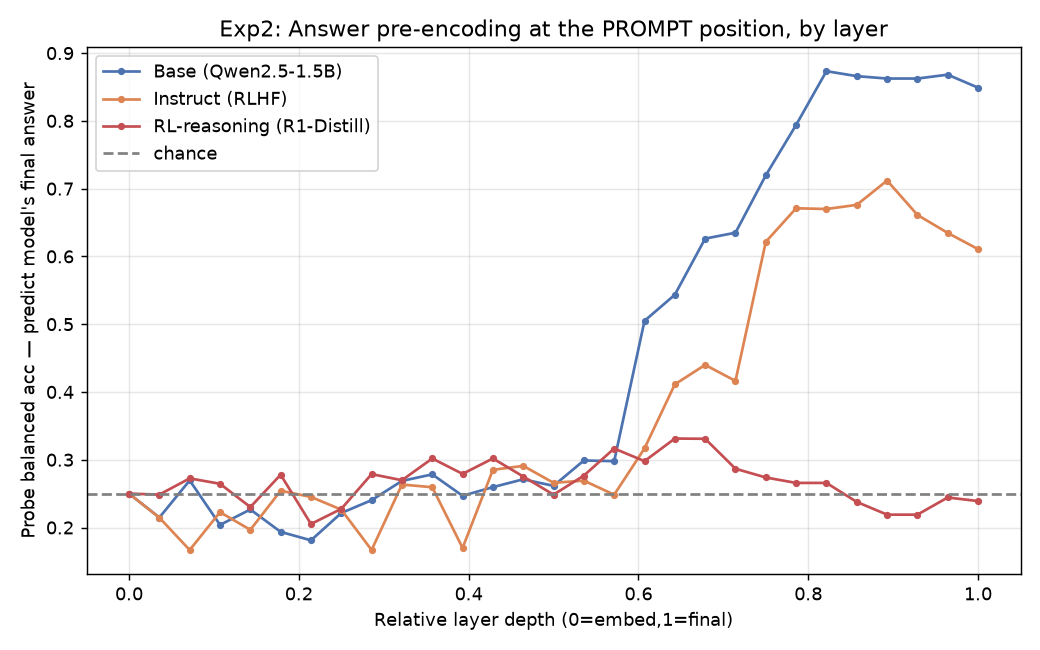
\includegraphics[width=\textwidth]{figures/exp2_layer_sweep.png}
        \caption{Probe accuracy across layers (prompt position).}
        \label{fig:exp2_layer}
    \end{subfigure}
    \hfill
    \begin{subfigure}[b]{0.48\textwidth}
        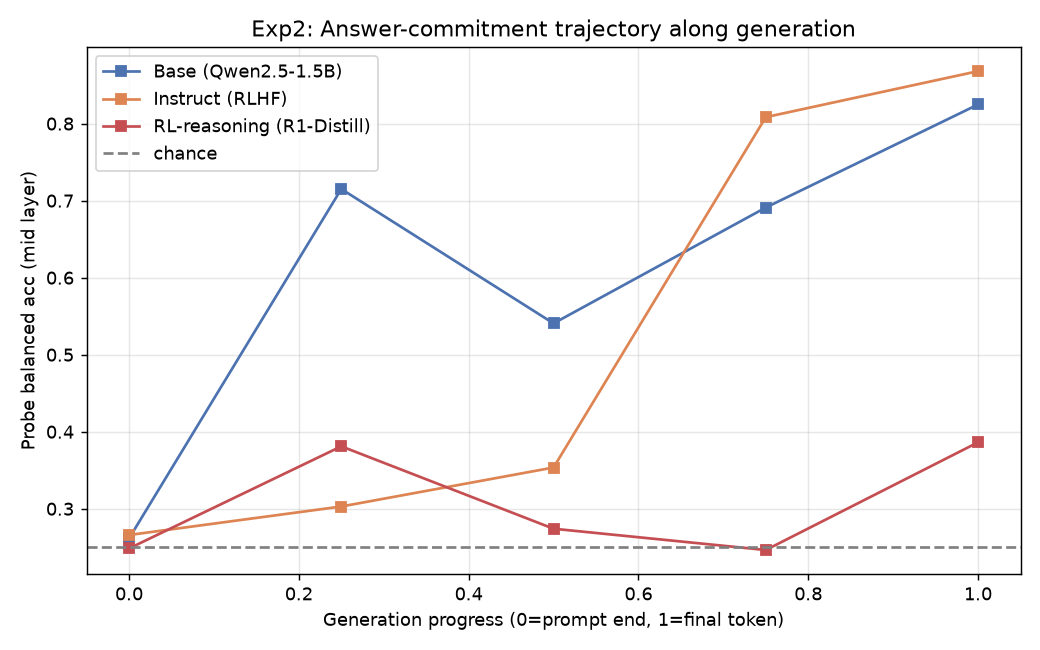
\includegraphics[width=\textwidth]{figures/exp2_timeline.png}
        \caption{Probe accuracy along the generation timeline.}
        \label{fig:exp2_time}
    \end{subfigure}
    \caption{Experiment~2 on \arc. \figleft The base model's answer becomes strongly decodable
    from the prompt hidden state in late layers (to $0.87$); \instruct reaches $0.71$; the
    reasoning model stays near chance ($0.25$) at every layer---its answer is not pre-encoded.
    \figright Commitment timing: the base model commits \emph{early} ($0.72$ by 25\% of
    generation), \instruct commits \emph{late} (rising only after 75\%), and the reasoning
    model's answer becomes decodable only at the very end. Commitment moves later with more
    post-training.}
    \label{fig:exp2}
\end{figure}

\figref{fig:exp2} shows where and when the answer becomes decodable. The base model's answer
emerges from the prompt representation in the late layers and is committed early in generation
(0.72 decodable by 25\% of the way through); instruct decides late (the curve rises only after
75\%); and the reasoning model decides through generation, its answer reaching decodability
only near the end. This is the clean, identically-measured contrast that the behavioral
results reflect.

\subsection{Experiment 3: rotating certainty redistributes uncertainty---in the base model}
\label{sec:res3}

\Tabref{tab:exp3} shows that holding a sub-fact certain reduces answer entropy for the base
model by $0.32$ bits when hop $A$ is fixed and $0.25$ bits for hop $B$, both strongly
significant ($p=1.8\times10^{-13}$); uncertainty is redistributed from the fixed hop onto the
rest of the question. The effect is marginal for instruct ($\sim$$0.08$--$0.09$ bits,
$p=0.019$) and \emph{absent} for the reasoning model ($\approx0$ bits, $p=0.84$): injecting
certainty about one hop does not move its answer entropy at all, because it reasons over the
whole question regardless. The cross-model gap is large (\base vs \rlm reduction:
Mann--Whitney $p=8.6\times10^{-9}$).

\begin{table}[t]
    \centering
    \caption{Experiment~3 on \strat ($N=120$; entropy in bits). $\Delta H$ is the entropy
    \emph{reduction} when a hop is held certain (larger $=$ more redistribution). Fixing a hop
    strongly redistributes the base model's uncertainty, marginally for \instruct, and not at
    all for \rlm. Largest redistribution per column in \textbf{bold}.}
    \label{tab:exp3}
    \begin{tabular}{@{}lcccccc@{}}
        \toprule
        \textbf{Model} & $H$(base) & $H$(+A) & $H$(+B) & $\Delta H$(+A) & $\Delta H$(+B) & \textbf{Wilcoxon $p$} \\
        \midrule
        \base     & 0.722 & 0.404 & 0.471 & \textbf{+0.318} & \textbf{+0.250} & $1.8\times10^{-13}$ \\
        \instruct & 0.420 & 0.341 & 0.327 & +0.079 & +0.093 & $0.019$ \\
        \rlm      & 0.555 & 0.607 & 0.528 & $-0.052$ & +0.027 & $0.84$ (n.s.) \\
        \bottomrule
    \end{tabular}
\end{table}

\begin{figure}[t]
    \centering
    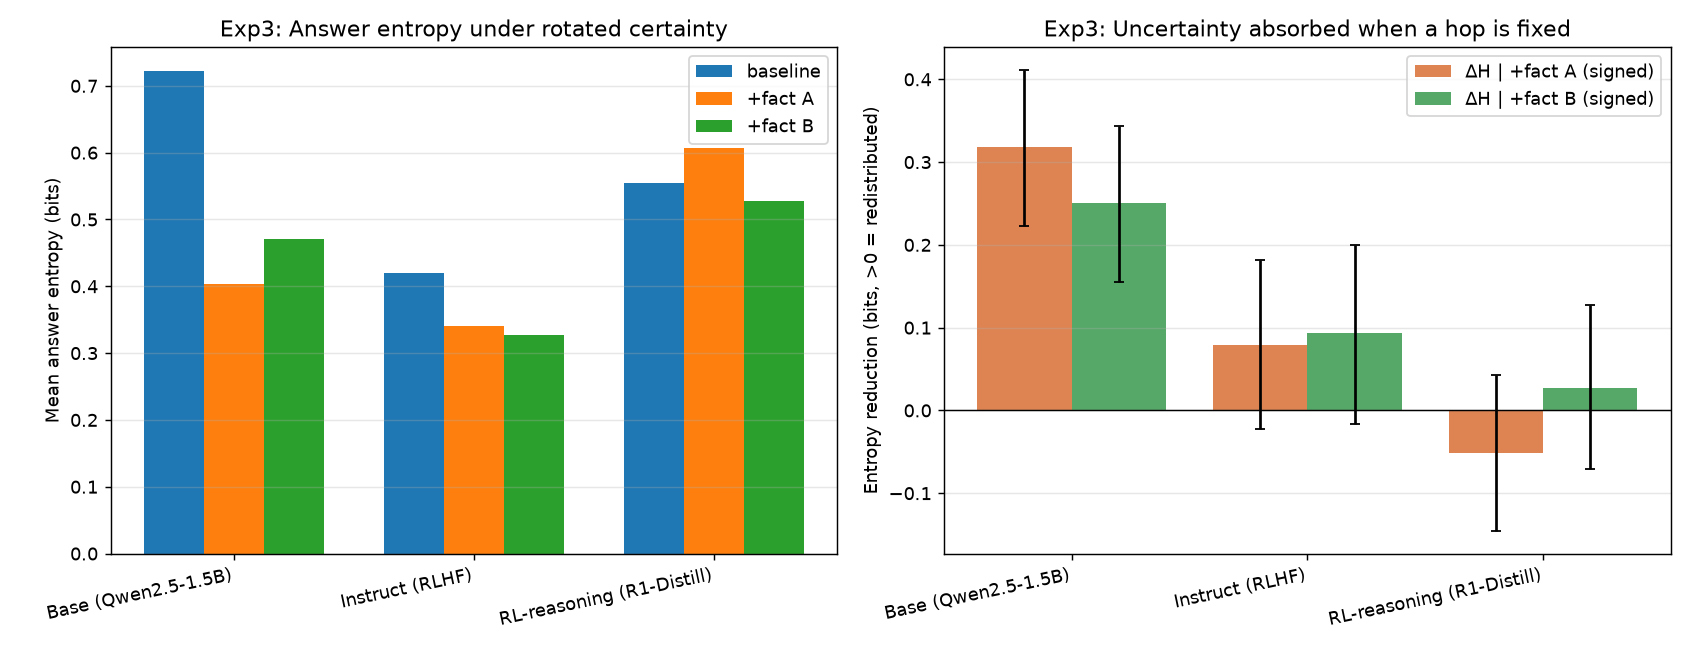
\includegraphics[width=0.6\linewidth]{figures/exp3_rotating.png}
    \caption{Experiment~3 on \strat. Answer entropy under \texttt{baseline}, \texttt{+A}, and
    \texttt{+B}. Fixing a hop redistributes uncertainty strongly for the base model (large,
    significant drop with CIs clear of 0), marginally for \instruct, and not at all for the
    reasoning model, whose answer entropy is robust to injected sub-fact certainty.}
    \label{fig:exp3}
\end{figure}
